\documentclass{article}

\usepackage{geometry}
\usepackage{amsmath}
\usepackage{graphicx, eso-pic}
\usepackage{listings}
\usepackage{hyperref}
\usepackage{multicol}
\usepackage{fancyhdr}
\pagestyle{fancy}
\fancyhf{}
\hypersetup{ colorlinks=true, linkcolor=black, filecolor=magenta, urlcolor=cyan}
\geometry{ a4paper, total={170mm,257mm}, top=10mm, right=20mm, bottom=20mm, left=20mm}
\setlength{\parindent}{0pt}
\setlength{\parskip}{0.3em}
\renewcommand{\headrulewidth}{0pt}

\rfoot{\thepage}
\fancyhf{} % sets both header and footer to nothing
\renewcommand{\headrulewidth}{0pt}
\lfoot{\textbf{Seleksi IEEEXtreme 17.0 ITB}}
\pagenumbering{gobble}

\fancyfoot[CE,CO]{\thepage}
\lstset{
    basicstyle=\ttfamily\small,
    columns=fixed,
    extendedchars=true,
    breaklines=true,
    tabsize=2,
    prebreak=\raisebox{0ex}[0ex][0ex]{\ensuremath{\hookleftarrow}},
    frame=none,
    showtabs=false,
    showspaces=false,
    showstringspaces=false,
    prebreak={},
    keywordstyle=\color[rgb]{0.627,0.126,0.941},
    commentstyle=\color[rgb]{0.133,0.545,0.133},
    stringstyle=\color[rgb]{01,0,0},
    captionpos=t,
    escapeinside={(\%}{\%)}
}

\begin{document}

\begin{center}

    
    \section*{Plum Blossom Garden} % ganti judul soal

    \begin{tabular}{ | c c | }
        \hline
        Batas Waktu  & 1s \\    % jangan lupa ganti time limit
        Batas Memori & 256MB \\  % jangan lupa ganti memory limit
        \hline
    \end{tabular}
\end{center}

\subsection*{Deskripsi}

Sunohara Shun adalah salah satu pengajar di sekolah Plum Blossom Garden. Murid-murid di sekolah tersebut sedang mempelajari mata pelajaran favorit mereka yaitu \emph{Matematika}. Untuk pelajaran hari ini Shun sudah menyiapkan sebuah graf berbentuk pohon yaitu graf terhubung tanpa cycle, dan pada graf tersebut setiap node memiliki sebuah nilai 1 digit.\\

Shun meminta masing-masing murid untuk memilih dua buah node a dan b lalu menyuruh murid untuk berjalan pada graf dari a sampai ke b namun setiap orang tidak boleh melewati node yang pernah ia kunjungi, dengan kata lain para murid akan berjalan dari a ke b mengikuti jalan terpendek pada pohon tersebut. Ketika berjalan, Shun meminta para murid untuk mencatat angka yang dilewati dan mencatat angka baru di posisi paling kanan setiap mencapai node baru. Setelah mendapat angka hasil perjalanan, Shun akan menyuruh murid untuk menentukan apakah nilai tersebut habis dibagi 11 atau tidak. Kokona, salah satu pengajar lain terpikir pertanyaan yang menarik yaitu berapa banyak pasangan a dan b dimana ketika dilakukan perjalanan akan didapat angka akhir yang habis dibagi 11. Bantu Kokona menghitung banyak pasangan a dan b dimana ketika dilakukan perjalanan akan didapat angka akhir yang habis dibagi 11

\subsection*{Format Masukan}

Baris pertama terdiri dari satu bilangan bulat positif $N (1 \leq N \leq 10^5)$, yang merupakan banyaknya node yang ada pada pohon.\\

Baris kedua terdiri dari N bilangan bulat positif $A_{i} (0 \leq A_{i} \leq 9, 1 \leq i \leq N)$, yang mana $A_{i}$ merupakan nilai bilangan yang terdapat pada node i.\\

N-1 baris selanjutnya terdiri dari dua bilangan bulat positif $u, v (1 \leq u, v \leq N)$, yang merupakan edge yang menghubungkan node u dan v pada graf, sudah dipastikan graf akan berbentuk pohon.

\subsection*{Format Keluaran}

Keluarkan sebuah bilangan bulat positif yang merupakan banyak pasangan a dan b dimana ketika dilakukan perjalanan akan didapat angka akhir yang habis dibagi 11.

\begin{multicols}{2}
\subsection*{Contoh Masukan}
\begin{lstlisting}
6
0 3 3 3 5 2
1 2
2 3
3 4
2 5
5 6
\end{lstlisting}
\columnbreak
\subsection*{Contoh Keluaran}
\begin{lstlisting}
13
\end{lstlisting}
\vfill
\null
\end{multicols}

\subsection*{Penjelasan}
Contoh graph pada soal adalah sebagai berikut \\
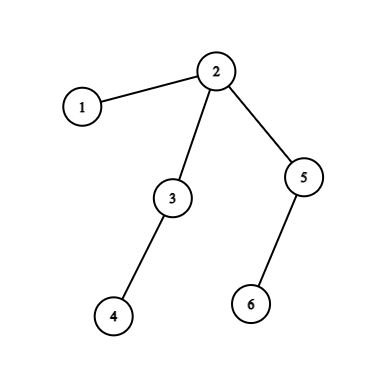
\includegraphics[scale=0.6]{graph} \\
Untuk contoh hasil angka yang didapat setelah melakukan traversal adalah\\
(3, 5) = 335\\
(1, 2) = 03 = 3 (angka nol yang berada di depan dihapuskan)\\
Untuk setiap pasangan (a,b) yang hasil angkanya habis dibagi 11 adalah sebagai berikut\\
1. (1, 1)\\
2. (1, 3)\\
3. (1, 6)\\
4. (2, 3)\\
5. (2, 6)\\
6. (3, 2)\\
7. (3, 1)\\
8. (3, 4)\\
9. (4, 3)\\
10. (4, 6)\\
11. (6, 2)\\
12. (6, 1)\\
13. (6, 4)


\end{document}